\chapter{Experiments using the magnetometer\label{ch:results}}

In this Chapter I present the main results on measurements of the
properties of the magnetometer, optimization studies, and applications
of the magnetometer to characterize magnetic fields.  The main studies
that are presented are:
\begin{itemize}
\item Measurements of magnetic fields over long timescales using FID mode.
%  Conclusion: fields drift over time.  Question: how much is due to
%  magnetometer drift vs. other sources?
\item Adjustment of the pump and probe timescales in order to measure
  the field faster.
%  Allowed us to measure faster.
\item Magnetometer drift compared with drifts in the coil current and
  room temperature.  This study aimed at finding sources of drifts.
%Conclusion: neither drift seems
%  particularly correlated with field drift over long time periods.
%  Temperature stability seems quite good, consistent with Michi's
%  thesis.  Side conclusion: when field {\bf only} is changed, the
%  magnetometer responds as expected.  Implies that magnetometer works
%  well at sensing small changes in field, at least on shorter
%  timescales.
\item Studies of degaussing, which in part tell the story of our
  degaussing development and learning.  This includes studies of:
%with multiple goals, telling the story of
%  our degaussing
  \begin{itemize}
    \item the degaussing setup and testing it near zero field
%we set up the
%      system, we tested mainly sample rate (related to number of
%      oscillations) stated to be important in Thiel et al.  We found
%      that if the innermost shield was already degaussed that
%      additional poor/rapid degauss did not screw it up as badly as we
%      expected, until degaussing was very rapid.
    \item initial operations at non-zero field, and
%Ramp field to large values, without
%      degaussing was bad.  After degaussing was better.
    \item final degaussing procedure, in which degaussing the next to
      innermost shield was studied.
  \end{itemize}
\item Studies of laser locking and tuning, and the requirements on
  tune stability
%again multiple goals:
%  \begin{itemize}
%    \item Lock point or laser seems to drift over time.  See ``Drift
%      is about 120 pT'' where statistical error gets worse.  Also
%      would lose lock sometimes.  We think this may be due to PBS.
%    \item Other concern is whether drift of lock affects measured
%      field.  Studied by ``manual locking'' and found not to be
%      important.  Lock drift does not affect measured field drift very
%      much, but does affect statistical precision of magnetometer.
%  \end{itemize}
\item Studies pushing below 1~pT in an individual FID measurement.
  This includes adjustment of the pump and probe powers, and lock-in
  amplifier settings.  As will be shown, this study revealed problems
  in the procedures used to determine the precession frequency at such
  high precision and suggests avenues for further study.
%But when
%  we improved the statistical precision significantly, we began to run
%  into systematic errors in frequency measurement.  This led us to
%  study additional errors related to lock-in amplifier settings.
%  Future work is to finalize these studies in order to further reduce
%  the errors
\item Finally, I show my studies which revealed a way to use FID mode
  to measure transverse fields.
%Further work is
%  required to push to nT-scale transverse fields relevant for
%  typ.~unmeasurable gradients that enter $\delta_T$ correction in Hg-n
%  signals in nEDM experiments.
\end{itemize}
Each study will now be presented in turn and conclusions will be
summarized in Chapter~\ref{ch:conclusion}.

% Belongs in Magnetometer Literature Review Chapter 2?

%. In the case of AM NMOR, high-field
%resonance occur in addition to the regular zero-field resonance. The
%optical properties of the medium are being modulated at twice the
%Larmor frequency. In the case of strong external magnetic field, the
%dynamic Stark effect limits the sensitivity of NMOR based atomic
%magnetometry by reducing the accuracy of the field measurement. The
%advantage of using AM NMOR method is that it can reduce the Stark
%effect because light frequency is not affected by amplitude
%modulation\cite{gawlikoptical}. In AM NMOR, It is easily possible to
%control the number and amplitudes of the high field resonances by
%using the square wave modulation of light intensity.




\section{Long-term FID measurements\label{sec:long-term FID measurement}}

A forced-oscillation scan or an acquisition of a single FID give a
measurement of the magnetic field within a relatively short time
period ($<1$~s).  For nEDM experiments, it is important to get
information about the change in the average magnetic field over time
periods of 100~s and longer.

In order to study the fluctuations and drifts in the magnetic field
over time, and to search for possible drifts in the magnetometer
itself, repeated measurements of FID's were made and recorded.

%long
%term data was taken in the FID mode.
During this long term process the laser frequency was tuned for
maximal FID amplitude, and locked using the DigiLock 110 module.  In
order to observe the FID signal, a Tektronix DPO 2014 oscilloscope was
connected to X and Y output of output of lock-in amplifier. A Python
script was used to set up the function generator and to trigger data
acquisition using the oscilloscope. The same script is also used to
transfer data continuously from oscilloscope to the computer.  For
further data analysis another Python script was used to process each
FID.  A least-squares fit was done for each FID for each X and Y pair.
The measured oscillation frequency of the decaying oscillating signal
was then convert to magnetic field using Equation~(\ref{eq:field}).

{\bf what are all the other settings of the magnetometer for these
  runs?  pump power is about 40$\mu$w,  pump time is 0.49~s,  probe power is about 22$\mu$w,  probe time is 0.5~s,  lock-in
  frequency is 1929.5 Hz , AOM frequency is 2038 Hz, lock-in time constant is 300$\mu$s...}

\begin{figure}%[h]
\centering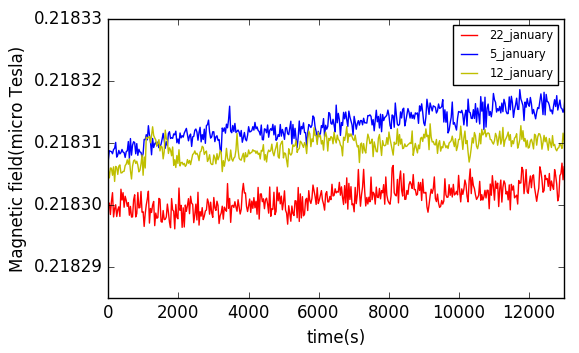
\includegraphics[width=0.85\linewidth]{figures/field_3_day}
\caption{Magnetic field recorded over 4 hours on three different
  days. The observed field drift is similar ($\sim 15$~pT) for each
  day.\label{fig:long-term-field}}
\end{figure}

Fig.~\ref{fig:long-term-field} shows the magnetic field recorded over
4 hours on three different days. Each data points in the graph
corresponds to a single FID measurement.  The observed field drift is
similar ($\sim 15$~pT) for each day.  The measurement was conducted at
0.2 $\mu$T magnetic field.

\begin{figure}%[h]
\centering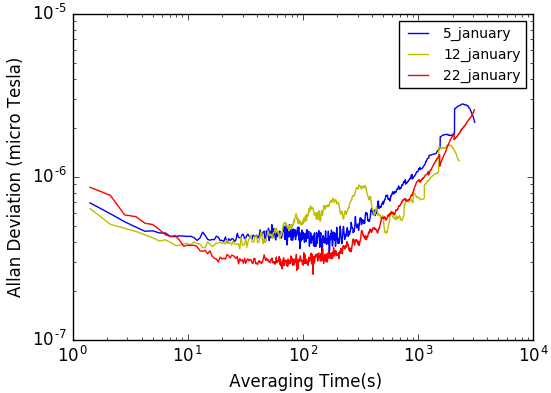
\includegraphics[width=0.8\linewidth]{figures/field_3_day_allan.png}
\caption{Allan deviation of recorded magnetic field vs.~averaging time
  for the time-series data presented in in
  Fig.~\ref{fig:long-term-field}.\label{fig:allan_deviation}}
\end{figure}

The Allan deviation was used to further quantify the long-term
stability~\cite{doe:website2} (see also Appendix~\ref{cite:appendix}.
Allan deviations characterize changes in the measured quantity when
the data are averaged on different timescales.  When the data behave
statistically on short timescales, the Allan deviation is equal to the
standard deviation.  If drifts occur, normally on longer timescales,
the Allan deviation grows linearly with a slope that $1/\sqrt{2}$
times the slope of the drift in time.

Fig.~\ref{fig:allan_deviation} shows the Allan deviations of the
measurements field presented in Fig.~\ref{fig:long-term-field}.  The
minimum in the Allan deviation occurs when statistical behavior is
overtaken by drift.  Fig.~\ref{fig:allan_deviation} shows that this
transition generally occurs after 10-60~s of averaging, corresponding
to a precision in magnetic field of 300-500~fT at the Allan minimum.

For an nEDM experiment, the goal precision is $\sim 20$~fT for the
average field over as measured over the 100~s neutron free-precession
measurement cycle.  This is not likely to be equivalent to the Allan
deviation minimum of our one magnetometer, because the long-term drift
is driven in part by the drift of the magnetic field within the
shield.  The goal of subsequent work was:
\begin{itemize}
\item to attempt to identify some of the sources of drift.  This
  included searching any sources that might be caused by the
  magnetometer itself, but also included the effects of
\item to improve the single FID performance so that fields could be
  measured faster.
\end{itemize}
In terms of the Allan deviation, it means trying to move the Allan
minimum lower and to the right.

\section{Optimization of cycle time} 

The goal of this optimization study was to reduce the cycle time
without sacrificing too much precision in the single-FID frequency
measurement.  If more measurements can be made more quickly, the
precision of the magnetometer over time would be improved.

\begin{figure}
\centering
\begin{subfigure}[b]{0.46\textwidth}
  \centering
  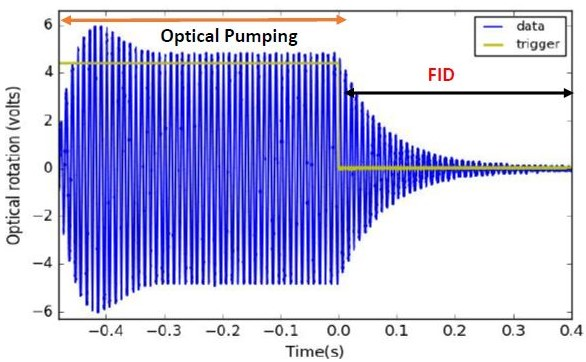
\includegraphics[width=\textwidth]{figures/Capture}
  \caption{}
  \label{fig:pump-long}
\end{subfigure}
\hfill
\begin{subfigure}[b]{0.45\textwidth}
  \centering
  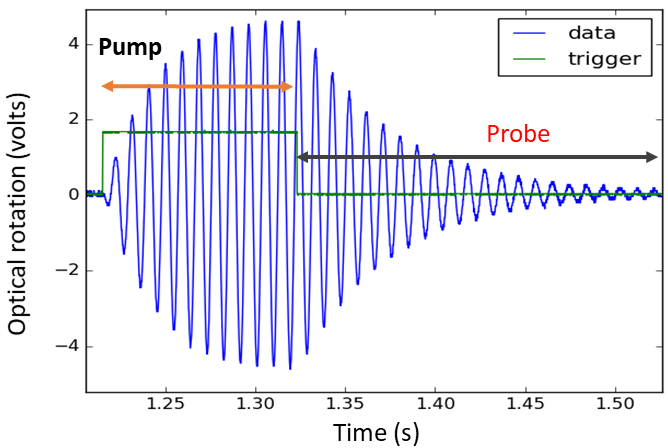
\includegraphics[width=\textwidth]{figures/FID_optimized.png}
  \caption{}
  \label{fig:pump-short}
\end{subfigure}
\caption{(a) FID signal for pump time 0.49~s and probe time 0.4~s. (b)
  FID signal for pump time 0.1~s and probe time 0.2~s.  Both
  measurements were conducted at $0.2~\mu$T magnetic field.}
    \label{fig:pump-time}
\end{figure} 


During this study the magnetometer was operated in FID mode at
0.2~$\mu$T field.
%A complete cycle of FID measurement consist of a
%pump time followed by a probe time.  Pump time represents the time
%atoms take to generate a polarized ground state. In this study we were
%trying to study how long the optical pumping of Rb atom should have
%continued in order to generate an alignment and optical pumping for
%long time does make any difference in measuring magnetic field
%precisely or not.
An example of our initial settings is shown in
Fig.~\ref{fig:pump-long}.  The pump time is 0.49~s and the probe time
is 0.4~s.  The amplitude of the differential photodiode signal is seen
to saturate well within 0.1~s.  The coherence time, indicated by the
decay time of the oscillating signal, is about 0.06~s.
Fig.~\ref{fig:pump-short} shows a more optimized the FID signal for
0.1~s pump time and 0.2~s probe time.

\begin{figure}%[h]
  \centering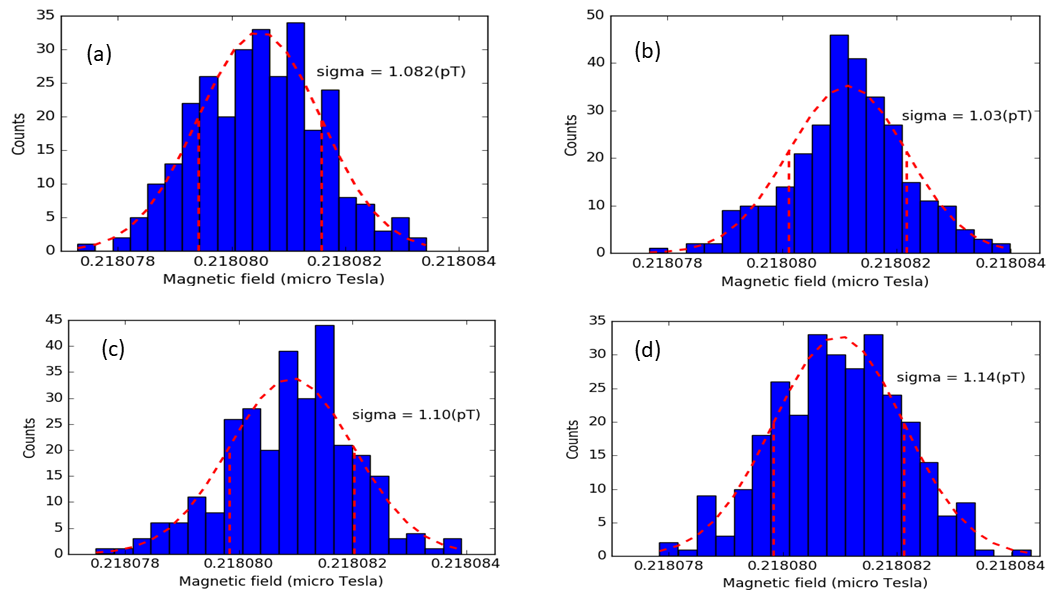
\includegraphics[width=0.75\linewidth]{figures/pump_time}
  \caption{Histograms of measured B-field for different pump times,
    {\bf for a measurement time of 300~s}. {\bf (a) is a pump time of
      0.49~s (b) is a pump time of 0.39~s (c) is a pump time of 0.2~s (d) is a
      pump time of 0.1~s.  The probe time in each case is 0.25~s.  The number
      of measurements taken in each case is therefore (a) 405 (b) 468
      (c) 666 (d) 857.  The standard deviation of each set of
      measurements is indicated in the respective
      figure.}\label{fig:different-pump-time}}
\end{figure}

In Fig.~\ref{fig:different-pump-time} a histogram of measured magnetic
fields by making subsequent measurements over 300~s is shown for
different pump times.  {\bf Which one is which? What is in the figure?
  The longer pump time is 0.49 s and the shorter one is 0.1 s.  What
  is the probe time.  How many measurements appear in each graph?}

From Fig.~\ref{fig:different-pump-time}, the pump time, when varied
over this limited range, does not strongly affect the precision of the
individual FID measurements.  {\bf However, it allows us to take
  measurements faster.  How much faster?  You need to say the times
  and/or how many measurements.}
  
%  However for our Rb magnetometry setup the
%shortest pump time 0.1 s because 0.1 s is the minimum time atoms need
%to get aligned for making a coherence state after interacting with
%laser beam. Since the amplitude of FID NMOR signal reach it's maximum
%while atoms are in coherence state. Thus It is easy to understand
%coherence state is ready or not by observing the signal amplitude.

It is not surprising that the precision does not change much because
the amplitude of the differential photodiode signal during the pump
phase has saturated.

%In Fig.~\ref{fig:pump-long} the optical pumping is done for 0.49 s
%while signal amplitude reach its maximum over 0.1 s and after that
%signal amplitude remains unchanged till 0.49 s. In this case there is
%no point to pump more than 0.1 s. Same situation happens about probe
%time. If signal amplitude decays so quickly there is no point to set
%longer probe time. By optimizing pump and probe time we can speed up
%data acquisition system. After optimization for a single FID scan it
%only takes 0.35 s without losing any information. By using this faster
%data acquisition system it is possible to record multiple FID run with
%in a short period of time which is helpful to gather more information
%about magnetic field environment and helpful to achieve statistical
%precession.


\section{Magnet field compared with current in the $z$-coil}

\subsection{Field drift compared with current drift}

The idea was to determine the impact of possible current drifts.
  
An Agilent B2962A power supply was used to supply DC electrical
current to the $z$-coil.

\begin{figure}%[h]
\centering
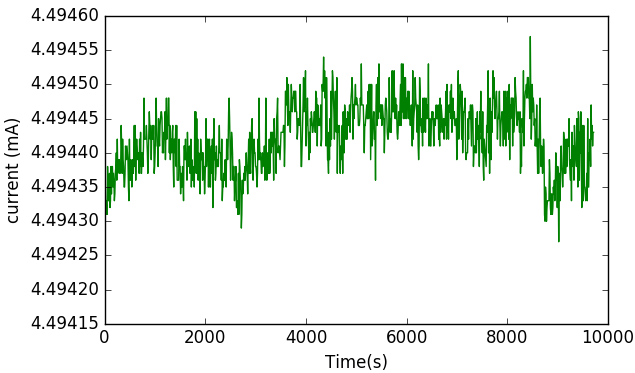
\includegraphics[width=0.6\linewidth]{figures/current}
\caption{Recorded current over 10000~s using Keithley multimeter %Agilent B2962A power source
{\bf How is this measured?  What is recorded by the power
    source?}.\label{fig:current} }
\end{figure}

Fig.~\ref{fig:current} shows the current {\bf measured how?} supplied
to the $z$-coil over a {\bf measurement} period of 10000~s.  The
current was set to 4.5~mA {\bf what is the correct value?  Was it set
  to 4.49440, or 4.494400, or 4.4944000 mA?  If not, what is wrong
  with the power supply?} in order to achieve a magnetic field of
0.2~$\mu$T.  The maximum current excursion during the measurement
period was 30~nA.

%\begin{figure}%[h]
%\centering
%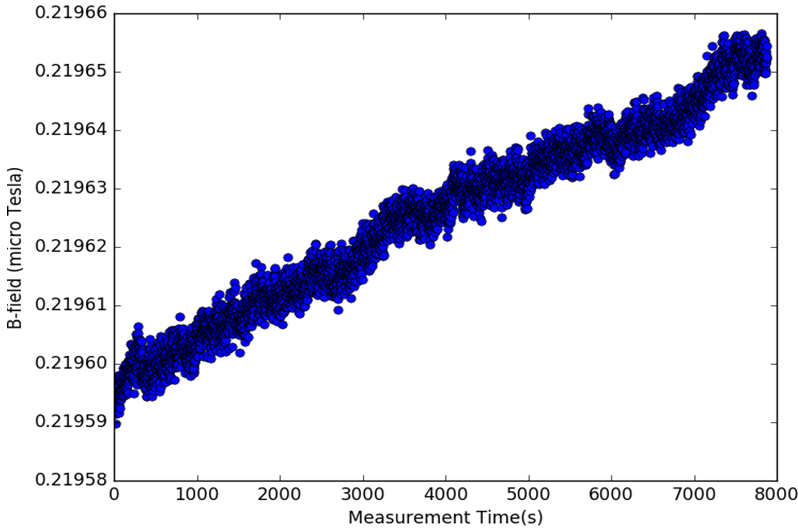
\includegraphics[width=0.6\linewidth]{figures/field_current_study.png}
%\caption{Magnetic field vs. time.\label{fig:field_current} }
%\end{figure}


\begin{figure}
  \centering
  \begin{subfigure}[b]{0.65\textwidth}
    \centering
    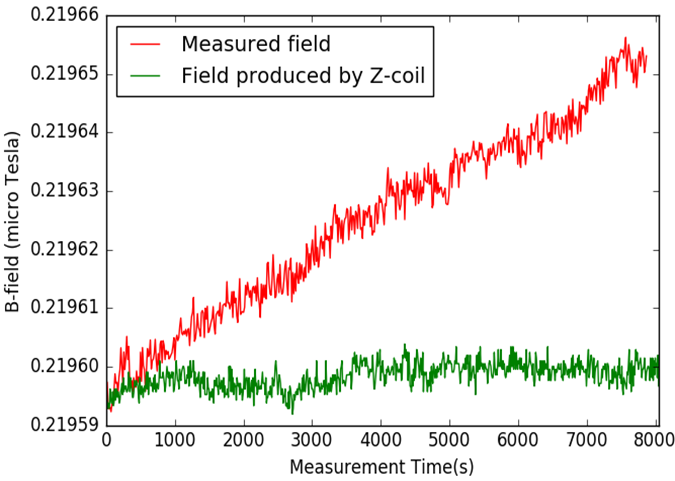
\includegraphics[width=\textwidth]{figures/field_coil_current.png}
    \caption{}
    \label{fig:field_measure_and_produced}
  \end{subfigure}
  \begin{subfigure}[b]{0.65\textwidth}
    \centering
    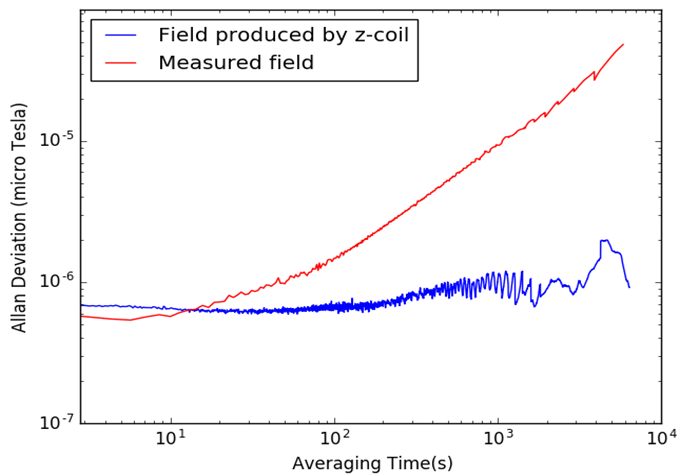
\includegraphics[width=\textwidth]{figures/field_current_allan_plot.png}
    \caption{}
    \label{fig:allan_plot}
  \end{subfigure}
  \caption{(a) Measured and produced magnetic field vs. time. {\bf
      what is each curve?}  (b) Allan deviation of field. {\bf why are
      the colors not the same as the above curves?  Why is the legend
      in the opposite order?}}
  \label{fig:current_vs_field_allan_deviation}
\end{figure} 

Fig.~\ref{fig:field_measure_and_produced} displays the magnetic field
measured by the magnetometer over the same period.  {\bf list all
  settings, lock-in time constant, laser power, lock-in frequency,
  magnetometer measured frequency, etc.}

produced by z-coil(green line) and measured field (red line) by
running the magnetometer in FID mode over 8000 s. The field generated
by z-coil is calculated by converting measured current to field with
coil constant of z-coil {\bf what value of the coil constant was used?
  According to my calcuation it is 0.048860236 uT/mA... this is not
  the same as the 48 nT/mA which you say it is...} (discussed in
Section~\ref{sec:internal-coil}).  At $t=0$ both fields {\bf are
  forced to?} coincide {\bf are normalized at t=0 by adjusting the
  coil constant to be XXX?} but over time a linear drift can be seen
in measured field.  For better understanding of the stability of the
power supply, providing current to the $z$-coil, the Allan deviation
of the generated field and measured field has shown in
Fig.~\ref{fig:allan_plot}.  It can be seen from the figure that
current stability is better than typical measured field changes.

{\bf How is the coil current measured?  Why was the coil current
  measured for longer than the field?  Was the coil current averaged
  over the same time as each frequency measurement?  Why is the
  current noisier than the magnetometer for short averaging times in
  the Allan deviation?  How were the current and field data acquired?
  How were the data synchronized to one another in time?  How is the
  measurement time defined for the coil current?  Is it at the start
  of the FID measurement or the end of the FID measurement, or
  somewhere in the middle, or asynchronously?  For the FID
  measurements, which time is graphed?  The start, end, or half-way
  time, or at the 1/e time of the FID?  Please show the measured coil
  current in the next section as well for
  Fig.~\ref{fig:field-change}.}



\subsection{Change in magnetic field driven by change in coil current}

A study has been conducted to determine the field change by changing
the coil current by a known amount. The main objective of this study
is to check the Rb magnetometer performance on magnetic field
measurement. During this measurement coil current has been changed by
$\pm 0.001$~mA. As a result a field change of $\pm 50~\mu$T {\bf pT?}
has been observed. The laser frequency was locked to Rb transition
frequency and all other setting kept unchanged. During this study the
magnetometer has been operated in FID mode {\bf list all documented
  settings.  What was the lock-in time constant, lock-in frequency?
  Were both x and y data simultaneously fitted? %only x data was fitted
  pump time?  probe
  time?%pump and probe time are 0.5~sec and 0.5~sec respectively
  }.
\begin{figure}%[h]
\centering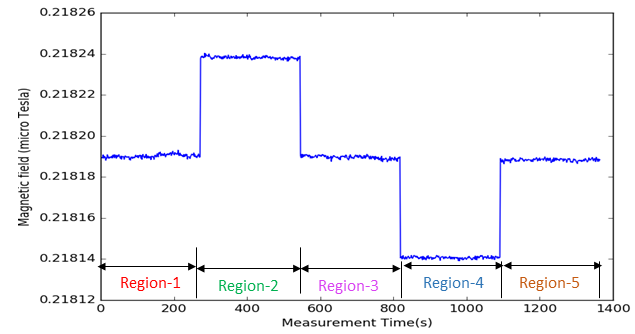
\includegraphics[width=0.7\linewidth]{figures/field_change_with_current}
  
\caption{The change in magnetic field  by changing coil current has been studied over 1400 sec. The blue line on different regions of the graph displays the measured magnetic field corresponding to the change in coil current. \label{fig:field-change}}
\end{figure} 
 
Fig.~\ref{fig:field-change} presents the magnetic field change over
time for different coil current. For better understanding
Fig.~\ref{fig:field-change} has been divide into five different
regions. In region-1 magnetic field has been recorded for 300 s while
the applied current to the Z coil was 4.5 mA {\bf do you mean
  4.500~mA?%  I mean 4.5000~mA
  How many digits of precision are possible in the current
  supply? }%6-digit. 
  Then in region-2 the applied current to the z coil has
been increased by 0.0010 mA {\bf sig figs?} i.e., total current 4.5010
mA {\bf sig figs?} and measured the magnetic field for another 300
s. It is clear from the figure that the field has been changed
instantly by 50 $\mu$T due to the changed coil current. Now in
region-3, the coil current has been reduced to 4.5000 mA {\bf sig figs?}
and measured field for 300 s. After that the coil current has been
decreased by 0.0010 mA. As a result the field also decreased by
50~$\mu$T in this region.  Finally in region-5 the coil current has
been set to 4.5000 mA again and observed the corresponing quick change in
field.

\section{Study the effect of room temperature in magnetic field} 

\begin{figure}%[h]
\centering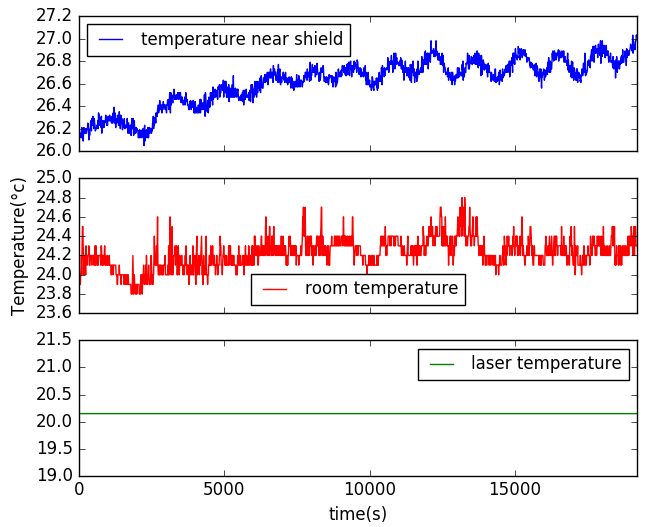
\includegraphics[width=0.8\linewidth]{figures/temp_.png}
\caption{Temperature measurement\label{fig:temperature-measurement}}
\end{figure}
Room temperature is measured using precision thermometer {\bf where?}
and laser temperature is measured from the output of the laser
temperature controller panel. The temperature on the magnetic
shielding {\bf where?  Why is it different than room temperature?% I think the reason is that the optics table is fully covered by heavy curtains which make this place warmer than rest part of the room. I also discussed it with Dave he also mentioned me the same reason.
} is
measured by a T-type thermocouple.  Since T- type thermocouple is
non-magnetic we use this specific type of thermocouple instead of
K-type.
 
  \begin{figure}%[h]
\centering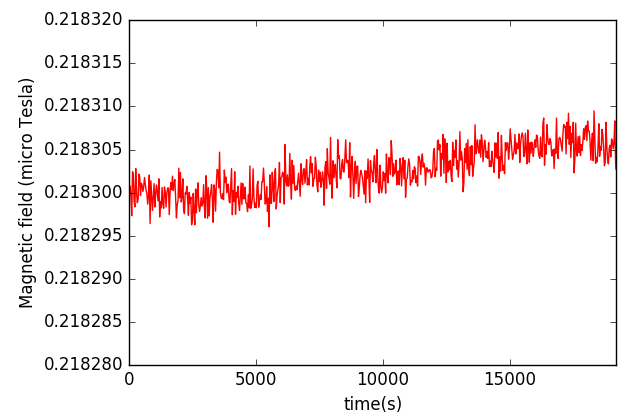
\includegraphics[width=0.8\linewidth]{figures/field_.png}
\caption{Field measurement\label{fig:field}}
\end{figure}

Fig.~\ref{fig:temperature-measurement} display the measured
temperature vs time.  During the measurement the laser temperature
(green line) remain unchanged which provide an indication about well
controlled laser diode temperature.  It can be seen from the figure
that room temperature fluctuation is 1\degree while temperature
outside of the magnetic shielding is about 0.8\degree.
 
Fig.\ref{fig:field} shows the magnetic field {\bf state all
  magnetometer settings} vs.~time while the temperature measurement
has taken place. In order to understand the correlation between
temperature change and field change, the measured field
vs. temperature has shown in Fig.~\ref{fig:field_vs_temp}. {\bf What
  was the data acquisition system for each device?  How were the data
  synchronized?% For room temperature measurement a precision themometer was connected to a Agilent 34410A/11A 6 ½ Digit Multimeter. A python script is used to configures the multimeter for a 2-wire RTD measurement, triggers the meter, and then transfers the reading to the computer via instrument output buffer. .
  }  It is clear from the graph that there is no obvious
of field drift dependency on temperature.
  
\begin{figure}%[h]
\centering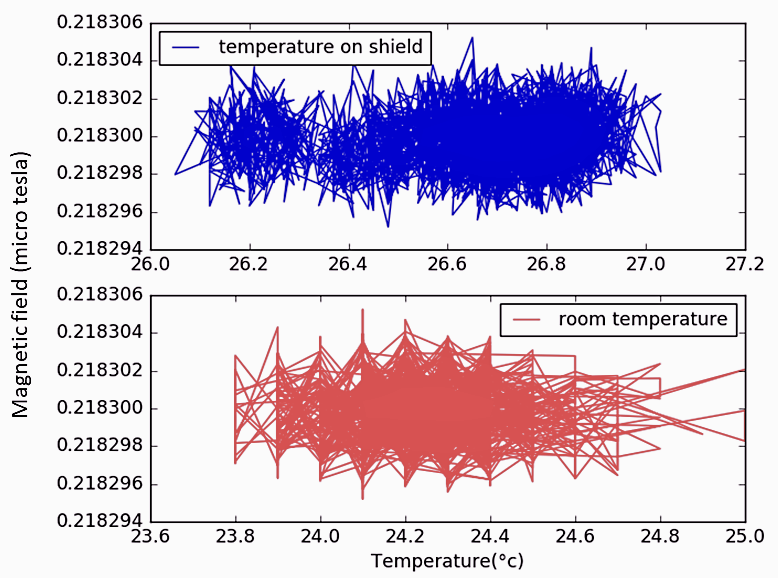
\includegraphics[width=0.6\linewidth]{figures/field_vs_temp.png}
\caption{Field vs. temperature\label{fig:field_vs_temp}}
\end{figure}
 
   
\section{Degaussing studies\label{sec:degaussing}}

\subsection{Initial tests using the magnetometer near zero field}

%different degaussing schemes(changing sample rate)
   
  
%Degaussing process is done in order to avoid the environmental
%perturbation and reduce any remnant field inside the four layer $\mu$
%metal magnetic shield \cite{doi:10.1063/1.2713433}. The setting for
%degaussing has shown in Table \ref{table:degaussing-setting}.  A
%detailed analysis of NMOR signal by changing the degaussing parameter
%could give us some information about the goodness of degaussing
%procedure. Toward this end, a study has been carried out to determine
%the dependency of the resonance width on the sample rate (see
%discussion on section \ref{sec:Degaussing}).

We used the procedure described in Section~\ref{sec:zerofield}.  To
remind the reading, the procedure is:
\begin{itemize}
\item Initiate degaussing in function generator.
\item Once complete, ramp the rheostat to zero and open the switch.
\item Pressing a button on the computer initiates the ramp of the
  $z$-coil, which calibrates the optical rotation to field.
\item Both the current in the $z$-coil and the differential photodiode
  signal are monitored at all times using an oscillscope.
\end{itemize}

%In this study, data was acquired by sweeping the magnetic field near zero field. Before each measurement degaussing the innermost layer of shield has done. During this measurement only one degaussing parameter, sample rate, was varied in order to study the effect of degaussing parameter on magnetic field measurement.  

\begin{figure}%[h]
  \centering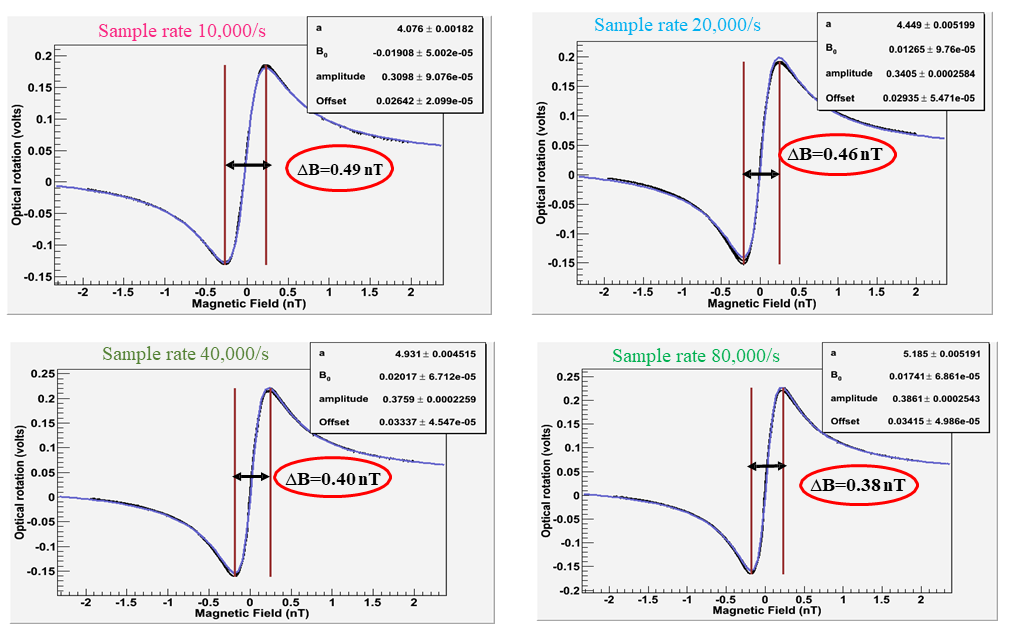
\includegraphics[width=\linewidth]{figures/sample_rate}
  \caption{ Optical rotation vs. measured B-field for different sample
    rate.  {\bf What order were the data taken in?% smaller sample rate to higher sample rate
    }  The numbers
    written in the red circles indicate the distance in magnetic field
    from the optical rotation minimum to the optical rotation maximum
    $\Delta B$, as deduced from the fit parameter $a$.  The fit
    parameter $B_0$ indicates the remnant field sensed by the
    horizontal offset of the dispersive shape, reported in
    nT.\label{fig:different-sample-rate}}
\end{figure}

Optical rotation as a function of magnetic field for different sample
rate has shown in Fig.~\ref{fig:different-sample-rate}.  Recall that
the sample rate determines the rapidity with which the $5\times 10^5$
individual samples of the linear degaussing envelope function are
stepped through.  A sample rate of 10,000/s therefore represents a
degaussing time of 50~s.  Since the carrier wave in all cases is
10~Hz, it means that 500~cycles were used.  The sample rate of
80,000/s represents a degaussing time of 6.25~s and 62.5 cycles.

It should also be noted that the data were acquired in order of
increasing sample rate, and that many additional degaussing sequences
were conducted which are not shown in
Fig.~\ref{fig:different-sample-rate}.

We had expected that larger sample rate would manifest itself as a
worse degaussing resulting possibly in worse magnetometer performance.q
Paradoxically, the resonance width $\Delta B$, the difference between
two peak of the dispersive curve, reduced as the sample rate was
increased.  It can be seen from Fig~\ref{fig:different-sample-rate}
that, the resonance width is about 0.49~nT for sample rate 10,000/s
and the resonance width is 0.38~nT for sample rate 80,000/s.  This is
likely an indication of a small change in the transverse fields or
generally an improvement the homogeneity of the field.  This is
consistent with the observation that the amplitude grows slightly with
amplitude, which is another indication of the field quality, all other
magnetometer settings being equal.

The remnant field $B_0$ is an indication of the average longitudinal
field (along the laser beam axis) and is within 20~pT of zero.  It
increased with the sample rate from a starting negative value to a
positive value.

The conclusion of this study was that additional degaussing, as long
as it has a reasonable number of cycles, tends not to affect the field
or to improve slightly the homogeneity of the field.  Generally the
field is always reduced below 20~pT.

%\begin{figure}%[h]
%\centering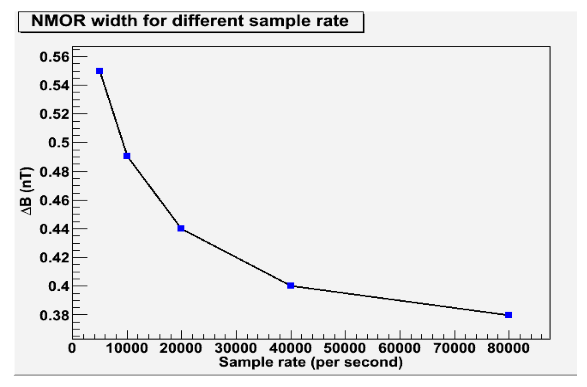
\includegraphics[width=0.6\linewidth]{figures/field_vs_sample_rate}
%\caption{Resonance width vs.~sample rate. Resonance width decreases
%  with increasing sample rate.  When the sample rate is 5000~samples/s
%  the observed resonance width is 0.55~nT. On the other hand the
%  resonance width is 0.38~nT for sample rate 80000
%  sample/s. \label{fig:resonance width vs. sample rate} }
%\end{figure}

%Fig~\ref{fig:resonance width vs. sample rate} shows the resonance
%width as a function of sample rate. Resonance width decreases with
%increasing sample rate.  It is obvious from the graph that the
%resonance width becomes narrower for larger sample rate.

\subsection{Measurements at 0.2~$\mu$T and initial studies of the effect of degaussing on field stability}
%Ramp field up/down 

The previous results implied that additional (even poor) degaussing
had little impact if the previous degaussing was done adequately.  To
address this, we began to do studies where the internal $z$-coil field
was purposely ramped to a large value, then reset to a low value for
measurements at non-zero field.

%A study has conducted by making the magnetic field environment bad
%inside the shielding intentionally by ramping the field from a lower
%value to higher value and observe any change in field drift. This
%study has done in 3-steps:
%  \begin{itemize}
%      \item take field measurement for about 2000 s without performing any degaussing.
%      \item Intentionally make the field environment bad and take field measurement for another 2000 s. No degaussing has done in this step also.
%      \item perform degaussing of the innermost shield and again measured magnetic field for 2000 s.
%  \end{itemize}

\begin{figure}
  \centering
  \begin{subfigure}[b]{0.425\textwidth}
    \centering
    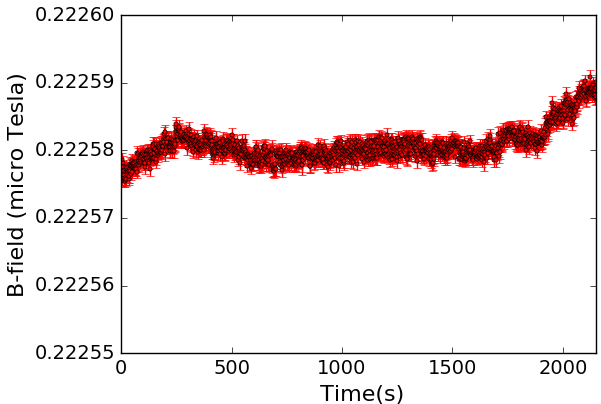
\includegraphics[width=\textwidth]{figures/ramp_1}
    \caption{}
    \label{fig:ramp-up}
  \end{subfigure}
  \hfill
  \begin{subfigure}[b]{0.42\textwidth}
    \centering
    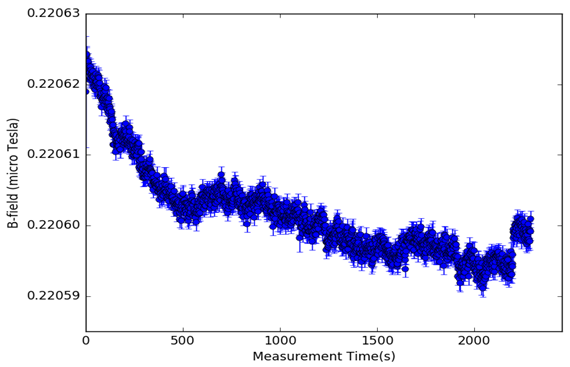
\includegraphics[width=\textwidth]{figures/ramp_2}
    \caption{}
    \label{fig:ramp-down}
  \end{subfigure}
  \begin{subfigure}[b]{0.42\textwidth}
    \centering
    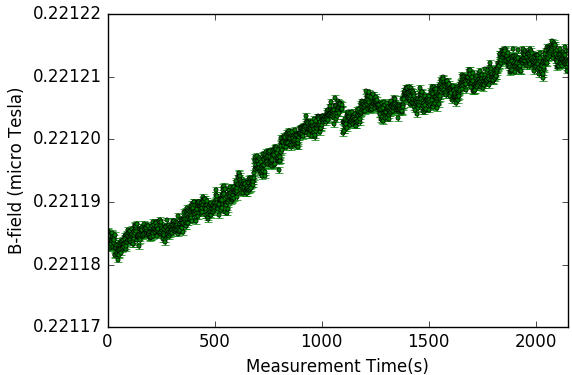
\includegraphics[width=\textwidth]{figures/ramp3}
    \caption{}
    \label{fig:degauss}
  \end{subfigure}
  \caption{{\bf Are these measurements conducted in time order from
      (a) to (b) to (c)?}% yes 
      FID signal at $B_z=0.2~\mu$T magnetic
    field.(a) no degaussing (b) Ramp $B_z$ from 0.2~$\mu$T to~10
    $\mu$T then again set it to 0.2~$\mu$T and collect FID signal (no
    degaussing). (c) study magnetic field stability after degaussing.}
  \label{fig:ramp-updown}
\end{figure}

Fig.~\ref{fig:ramp-updown} shows an example of such a study.  In all
three cases shown in Fig.~\ref{fig:ramp-updown}, the magnetometer
settings are similar.  Since the field changed in each measurement,
the magnetometer was retuned each time, principally the pump frequency
and the lock-in amplifier internal reference frequency.  {\bf What are
  the magnetometer settings?}
 % AOM frequency 2064 Hz and lock-in frequency 1950.2 Hz (fig:5.12(a))
 % AOM frequency 2059 Hz and lock-in frequency 1950.2 Hz (fig:5.12(b))
 % AOM frequency 2078 Hz and lock-in frequency 1950.2 Hz (fig:5.12(c))
  

In the 1st part of this study the magnetometer was operated in FID
mode at 0.2 $\mu$T field. The recorded magnetic field over 2200 s has
been showed in Fig \ref{fig:ramp up}. It can be seen from the figure
the magnetic field increase linearly for first 300 s then showed a
decrease in field. The field was pretty stable between 600 s and 1800
s and after that the field showed a rapid increase. The overall field
change is about 15 pT during the measurement. Data was acquired by
ramping $B_z$ from 0.2 $\mu$T to 10 $\mu$T then again set it to 0.2
$\mu$T and collect FID signal. By doing this field ramping we
intentionally perturb the magnetic field environment inside the
shield. After this field ramping the long term field measurement has
been conducted for another 2200 s. In this case, the field showed a
downward drift of about 35 pT. Thus field ramping has been changed the
magnetic field environment inside the magnetic shielding.
   
   \subsection{Effect of degaussing second innermost shield}
 
   
    The usual field was about 15 pT over 3000~s (discussed in sec \ref{sec:long-term FID measurement}) although  the reason behind field drifting problem was unknown.  After doing transverse field study (applying current to X and Y coil along with Bz coil) magnetic field environment became more unstable.  Fig \ref{fig:without DG} shows about 50 pT drift in magnetic field in 4000 s. In order to cancel background field inside shield degaussing innermost layer of $\mu$ metal is done but it doesn't help to solve field drift problem. During this study the lock-in reference frequency is set to 1938.5~Hz and lock-in time constant is 300$ \mu$s. Then degaussing the 2nd innermost layer of shield is done which solve the field drift problem. Since the end cap of the innermost shield layer is not in use some background field leaked into 2nd layer which was causing the drift in field. So by degaussing the 2nd layer of shield canceled background field and field becomes so stable (Fig \ref{fig:with DG}). During this two measurement all other setting remain unchanged only the degaussing of the 2nd innermost shield has performed.
   
  \begin{figure}
    \centering
 
    \begin{subfigure}[b]{0.45\textwidth}
        \centering
        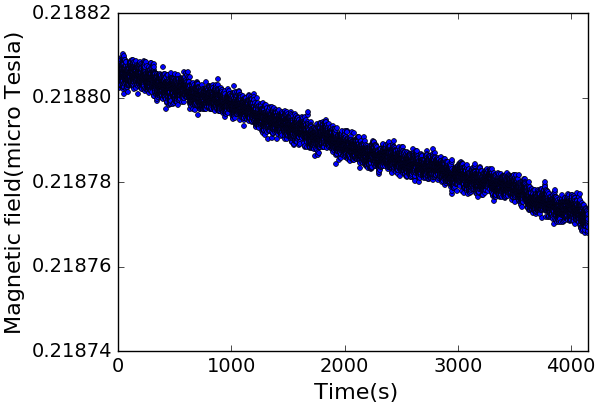
\includegraphics[width=\textwidth]{figures/before_degaussing}
        \caption{}
        \label{fig:without DG}
    \end{subfigure}
    \hfill
    \begin{subfigure}[b]{0.45\textwidth}
        \centering
        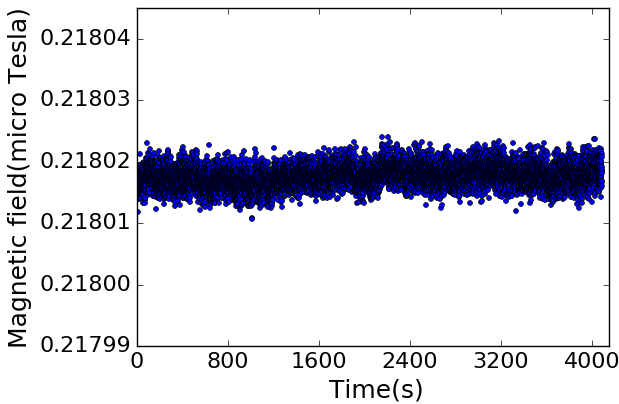
\includegraphics[width=\textwidth]{figures/after_degaussing}
        \caption{}
        \label{fig:with DG}
    \end{subfigure}
    \caption{ Magnetic field recorded over 3 hours. (a) The stability of magnetic field without performing any degaussing. A downward field drift of about 45 pT  has observed in this case (b) magnetic field stability after degaussing the 2nd innermost layer of magnetic shielding. Only a couple pT field drift has observed in this case. During this study the signal amplitude was pretty low($\sim$)3V} because of the low pump beam power(I think) or ther poor settings. As a result the precession width becomes wider(10~pT) while the usual is about 5~p 
    \label{fig:effect of DG}
\end{figure}
%   \end{itemize}
  
  \section{Laser tuning} 
   \begin{itemize}
   \item effect of careful tuning\\
	The main purpose of this study is to understand the importance of laser tuning on coherence life time of excited atoms. During the study optical pumping is done to polarize the rubidium atom and hence produce coherence state. When the laser light  is  exactly tuned to resonance with the atomic transition, the lifetime of coherence state becomes longer and the amplitude of resonance signal reaches its maximum. On the other hand coherence state decay  quickly when laser frequency detunes from atomic transition. In this case, the signal amplitude reduces due to frequency detuning.
	 \begin{figure}
    \centering
 
    \begin{subfigure}[b]{0.45\textwidth}
        \centering
        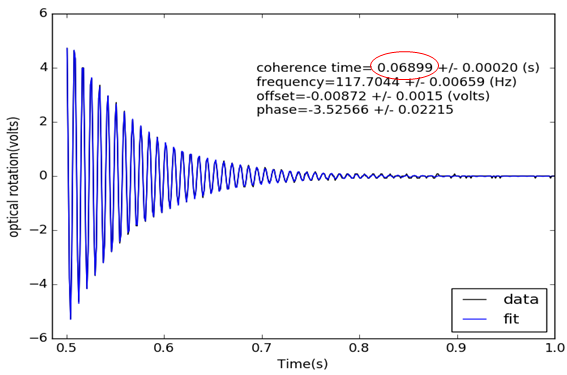
\includegraphics[width=\textwidth]{figures/perfect_tuning}
        \caption{}
        \label{fig:good tuning}
    \end{subfigure}
    \hfill
    \begin{subfigure}[b]{0.45\textwidth}
        \centering
        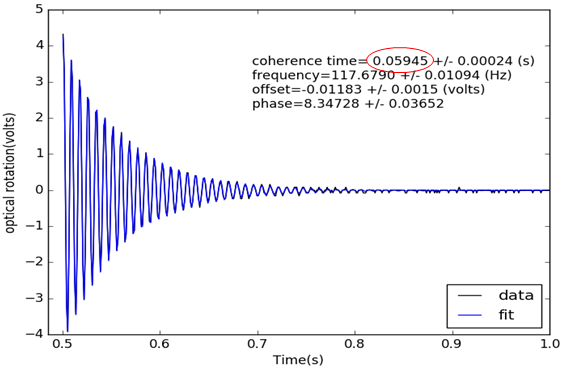
\includegraphics[width=\textwidth]{figures/bad_tuning}
        \caption{}
        \label{fig:bad tuning}
    \end{subfigure}
    \caption{(a) Recorded FID signal while laser is perfectly tuned to atomic transition frequency. (b) FID resonance signal when laser is slightly detuned from transition frequency.}
    \label{fig:effect of tuning}
\end{figure}
	
	Fig~ \ref{fig:effect of tuning} shows the effect of laser tuning on coherence lifetime. During this measurement the AOM frequency was set to 2.068~kHz and Lock-in frequency was 1.950~kHz.  For proper laser tuning the observed coherence time is 68 ms (Fig \ref{fig:good tuning}) whereas for bad tuning coherence time reduces to 59 ms (Fig \ref{fig:bad tuning}). On a fundamental level, the magnetometer actually measures the energy splitting between the Zeeman sublevels of the atomic ground state due to the magnetic field. The linewidth of such a spectroscopic measurement is given by the coherence lifetime $T_2$ of the atomic spins \cite{bib:Seltzer_thesis}
\begin{equation}
 \Delta B = \Delta\omega/\gamma  = 1/γ T_2
\end{equation}

The development of a sensitive magnetometer depends on achieving the maximum possible polarization lifetime.  For very short coherence time atomic spin depolarize quickly which limits the sensitivity of the magnetometer.
Since  longer coherence time and larger signal amplitude indicate better frequency precession and therefore precise field measurement it is very important to make sure the laser tuning has done carefully.
  
   \item problem with drift of tune
      \begin{figure}[h]
\centering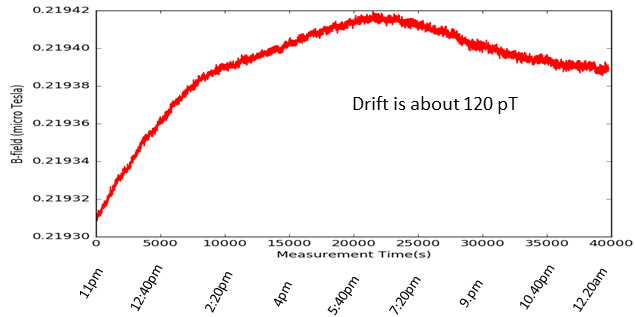
\includegraphics[width=0.6\linewidth]{figures/field_drift}
\caption{Magnetic field recorded over 12 hours.In this measurement the observed field drift is about 120 pT.\label{digilock field drift}}
\end{figure}
   For studying long term stability data was taken for about 12 hours. Laser was locked to D1 transition line of Rb using Digilock laser locking software. Fig \ref{fig:effect of tuning} shows 120~pT observed drift in magnetic field over 12 hours. Although DAVLL was in use laser frequency was not locked for 12 hours. As a result laser tuning moved due to mode hoping which causes the drift. The current laser locking system only works perfectly for maximum 4 hours. The possible reason for this mode hoping is the Polarizing beam splitting cube of our DAVLL system \cite{principles}. The disadvantage of using this type of PBS is that they show flaky optical behavior over longer times.

\item manual tuning\\
   During this study frequency of laser light is tuned to atomic transition maximize optical rotation. The laser tuning was adjusted manually time to time for maintaining same signal amplitude during measurement. The main objective of this study is to check the observed drift in field measurement is the real field drift or the magnetometer drift due to the mode hoping. Instability of laser locking system due to the poor performance of PBS which is used in DAVLL system is the probable reason behind this mode-hoping. According to Fig \ref{fig:amplitude manual tuning} we can say that during this measurement the amplitude of FID NMOR was pretty stable except small fluctuations over 20000 s . The observed small fluctuation is due to the manual adjustment while keeping the laser frequency tuned to atomic transition over long period of time. Obtaining stable signal amplitude is a indication that laser is not drifting to much. Although laser frequency was not drifting a lot during  the measurement, still there is a  drift in magnetic field (Fig \ref{fig:field manual tuning}). The overall drift is about 20 pT over 20000 s. So it can be conclude that the drift in laser frequency is not the main reason behind this induced field drift. 
   
    
   \end{itemize}
   \begin{figure}
    \centering
 
    \begin{subfigure}[b]{0.45\textwidth}
        \centering
        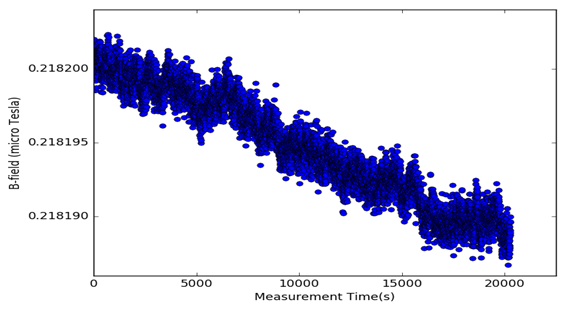
\includegraphics[width=\textwidth]{figures/manual_tuning}
        \caption{}
        \label{fig:field manual tuning}
    \end{subfigure}
    \hfill
    \begin{subfigure}[b]{0.45\textwidth}
        \centering
        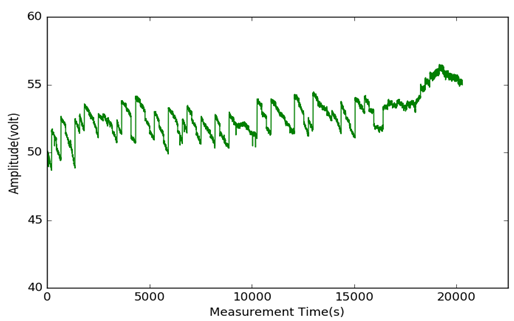
\includegraphics[width=\textwidth]{figures/amplitude_manual_tuning}
        \caption{}
        \label{fig:amplitude manual tuning}
    \end{subfigure}
    \caption{(a) magnetic field vs. time. (b) amplitude of recorded FID NMOR signal over 20000 sec. During this study laser tuning is maintained manually}
    \label{fig:manual tuning}
\end{figure}
\section{Systematic error check in frequency measurement in FID mode \label{sec:reference-frequency}} 
   \subsection{Optimization of pump and probe beam power} 
 A study has been performed to determine how optimization of the pump and probe beam power effect on precise field measurement.  During this study, the magnetometer has operated in FID mode.  A  linearly polarized probe beam has been used to analyze the spin response. 
  \begin{figure}
    \centering
    \begin{subfigure}[b]{0.7\textwidth}
        \centering
        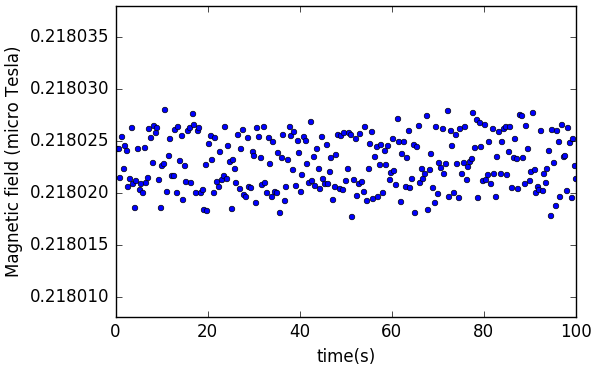
\includegraphics[width=\textwidth]{figures/beam_power_less}
        \caption{}
        \label{fig:power less}
    \end{subfigure}

    \begin{subfigure}[b]{0.7\textwidth}
        \centering
        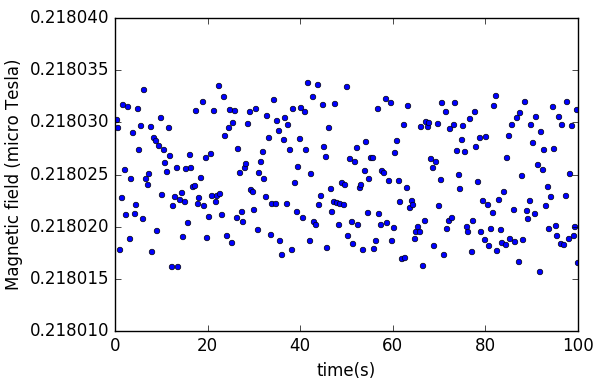
\includegraphics[width=\textwidth]{figures/beam_power_double}
        \caption{}
        \label{fig:power double}
    \end{subfigure}
    \caption{ Magnetic field as a function of time for different power of probe beam.(a) measured magnetic field with probe beam power 15 $\mu$w. Precession width is about $3.01$ pT (b) measured magnetic field with precession width $7.2$ pT for probe beam power 30 $\mu$w.}
    \label{fig:different probe power}
\end{figure}
%data colllected 13th August 2018
 
 In Fig \ref{fig:different probe power} the measured magnetic field has been displayed for two different  Probe beam power. Fig \ref{fig:power less} present the measured field over 100 s with 15 $\mu$W probe power while fig \ref{fig:power double} display the measured field over 100 s for probe power 30 $\mu$W. In both cases, the pump beam power has been kept unchanged ($5\%$ duty cycle). Each blue points in this graph represent a single FID scan. As can be seen from Fig \ref{fig:different probe power} the magnetic field is more scattered for high beam power. Precession width is about $7.2$ pT for probe beam power 30 $\mu$W while for low beam power(15 $\mu$W) the precession width is about $3.01$ pT. It can be concluded lower probe beam power is better for precession  magnetometry because the narrower the precession width more sensitive the magnetometer. Although low probe beam power is better for precise field measurement, it's hard to work with because of the dimness of light.
Table  \ref{table:Coherence time for different probe power} represent the coherence time for different probe power while the pump beam power was unchanged.
 \begin{table}%[h]
\centering
\begin{tabular}{|l  |c|c|}\hline
\textbf{Probe power($\mu$w)}    & \textbf{Coherence time(ms)}  & \textbf{Amplitude(Volts)}\\\hline
~~~~~~~~2 & 84 & 2.13   \\
\hline
~~~~~~~~5    & 82 & 2.11  \\
\hline
~~~~~~~~10   &  68 & 4.06 \\
\hline
~~~~~~~~15  &   59 & 5.8  \\
\hline
~~~~~~~~35  &   32 & 10  \\
\hline
\end{tabular}
\caption{Coherence time for different probe power\label{table:Coherence time for different probe power}}
\end{table}
 
 \begin{figure}
    \centering  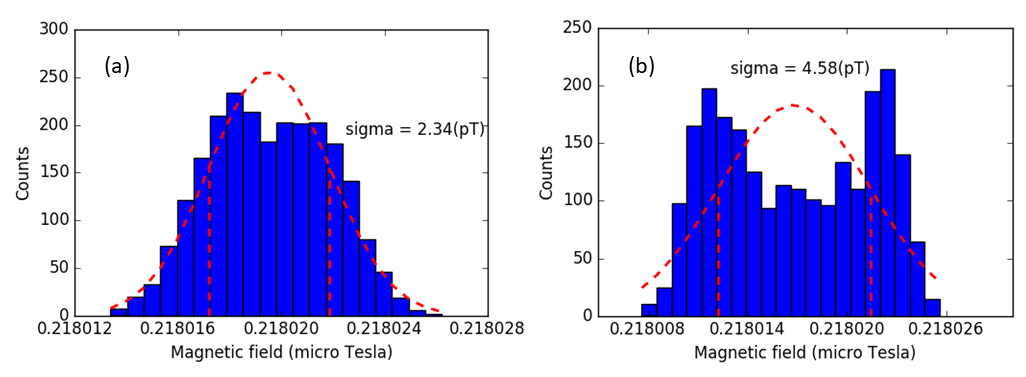
\includegraphics[width=\textwidth]{figures/pump_beam}
    \caption{ Magnetic field vs. time for different pump beam power. (a) measured magnetic field with duty cycle $5 \%$. Precession width is about $2.3$ pT (b) measured magnetic field with Precession width $4.6$ pT for  16 $\%$ duty cycle.}
    \label{fig:different pump power}
\end{figure}

Another study has been conducted to understand the influence of pump beam power on precession magnetometry. During this study, the probe beam power ($\sim$ 15 $ \mu$W) has kept unchanged while pump power has changed. In this measurement data has been acquired by running the magnetometer in FID mode. In FID mode amplitude modulation of pump beam has been done by using a AOM.  So the pump beam power can be change by changing the duty cycle of square wave modulation. When duty cycle is set to $5\%$ the pump beam power is 40 $\mu$W and for $16 \%$ duty cycle power is 128 $\mu$W. During this measurement the lock-in reference frequency was set to 1943.9 Hz while the AOM frequency was 2036 Hz. The histogram of measured magnetic field for different pump beam power has been showed in fig \ref{fig:different pump power}. The precession width (sigma) become larger for higher duty cycle while it becomes narrower for small duty cycle. In the case of 5$\%$  duty cycle precession width is about $2.3$ pT  (fig \ref{fig:different pump power}(a)) and for 16 $\%$ duty cycle the spread is about 4.6 pT (fig \ref{fig:different pump power}(b)). It is clear from the plot that, at higher duty cycle data points are not statistically distributed.  When a pump beam with a higher duty cycle is used  in precession magnetometry, the NMOR  signal amplitude increase accordingly. But it has been observed that error in frequency measurement also increases with higher signal amplitude which was not expected. A strong correlation between magnetic field and phase of the NMOR signal also has been observed for higher pump power. So it can be concluded that using higher duty cycle could induce more systematic errors in field measurement which led to the next study.


\subsection{How far the reference frequency of lock-in amplifier should set to measure field correctly}
  
  In FID NMOR the atomic sample is polarized once by optical pumping and then observed the spontaneous decay of excited atom while the pump beam is off. In order to capture the FID signal correctly, the reference frequency of lock-in amplifier is normally set to about 100 Hz apart from the resonance frequency. In this study we kept all other setting fixed only changed the Lock-in reference frequency and observed the effect of that on field measurement study. The measurement was conducted at $0.2 \mu$T field. 
   \begin{figure}
    \centering
    \begin{subfigure}[b]{0.4\textwidth}
        \centering
        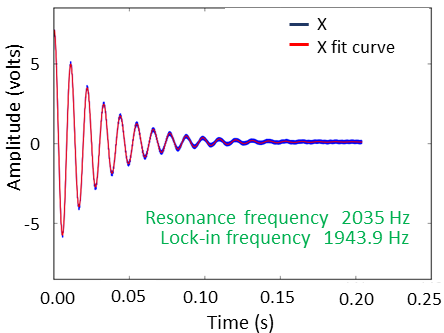
\includegraphics[width=\textwidth]{figures/reference_frequency1}
        \caption{}
        \label{fig:far from resonance}
    \end{subfigure}
    \hfill
    \begin{subfigure}[b]{0.4\textwidth}
        \centering
        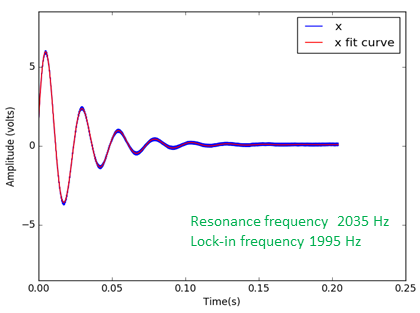
\includegraphics[width=\textwidth]{figures/reference_frequency3}
        \caption{}
        \label{fig: middle range}
    \end{subfigure}
    \begin{subfigure}[b]{0.4\textwidth}
        \centering
        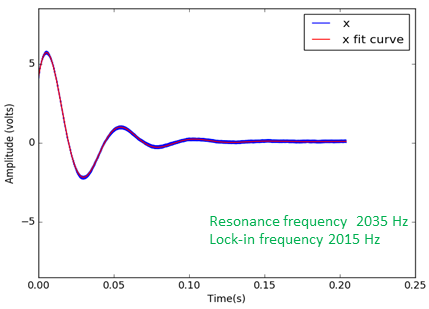
\includegraphics[width=\textwidth]{figures/reference_frequency2}
        \caption{}
        \label{fig:close to resonance}
    \end{subfigure}
 \caption{FID signal for different reference frequency of Lock-in amplifier while the resonance frequency was 2035 kHz.(a) reference frequency was set to 100 Hz far from resonance (b) difference between resonance and reference frequency is 40 Hz, (c) reference frequency was set to 2015 Hz while resonance frequency 2035 Hz. \label{fig:different reference signal}}
\end{figure}
  
  The FID signal for different reference frequency of Lock-in amplifier has shown in Fig \ref{fig:different reference signal}. In the case of Fig \ref{fig:far from resonance} the reference frequency of Lock-in was set to 1943.9 Hz (90 Hz far from resonance frequency). On the other hand for Fig \ref{fig:close to resonance} the reference frequency of Lock-in was set to 2015 Hz (20 Hz far from resonance frequency). In this study the resonance frequency is 2035 Hz. In Fig \ref{fig:field for different lockin ref freq} the measured magnetic field over 35 s for different lock-in reference frequency has shown. It is obvious from the plot that if we set reference frequency very close to resonance frequency magnetic field start to oscillate. The exact reason behind this observed field oscillation remains unknown. We are thinking that when lock-in reference frequency is set very close to resonance frequency the fit function might fail to fit data properly due to the less zero crossings. So it seems like a systematic effect on field measurement rather than a real fact.
   
\begin{figure}[h]
\centering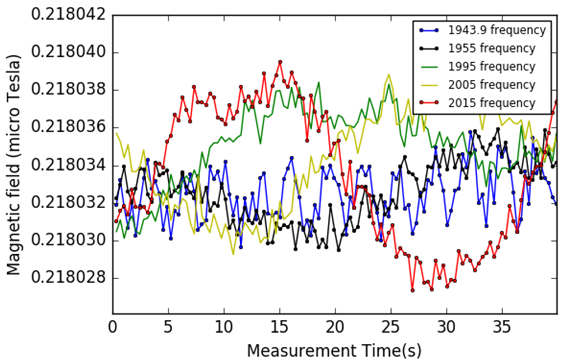
\includegraphics[width=0.8\linewidth]{figures/reference_frequency}
\caption{Measured magnetic field for different lock-in reference frequency. The red curve represents measured magnetic field when reference frequency was set to 2015 Hz which is 20 Hz far from resonance frequency. The blue curve shows magnetic field for lock-in reference frequency 1943.9 Hz.\label{fig:field for different lockin ref freq}}
\end{figure}
   

\begin{figure}[h]
\centering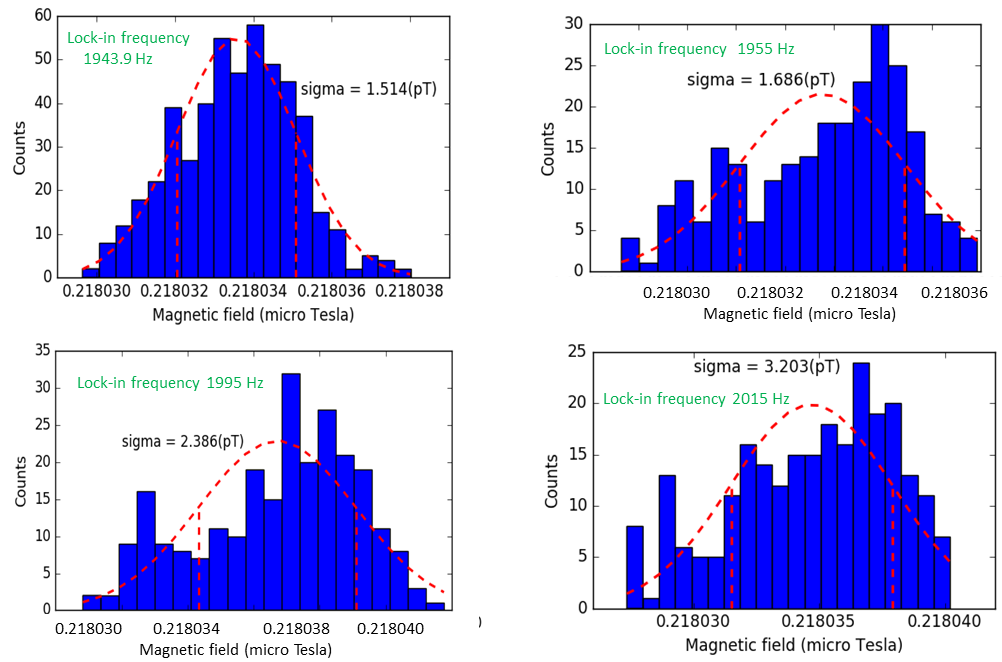
\includegraphics[width=0.8\linewidth]{figures/sigma_diff_lock-in_frequency.png}
\caption{Histogram of the measured magnetic field for different lock-in reference frequency.\label{histogram-of-diff-lock-in freq}}
\end{figure}

\begin{figure}[h]
\centering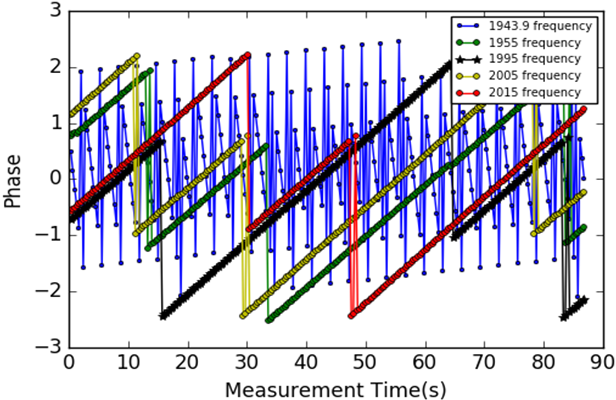
\includegraphics[width=0.8\linewidth]{figures/phase_vs_time.png}
\caption{Phase for different lock-in reference frequency.\label{phase_different_lock-in_frequency}}
\end{figure} 

 \begin{figure}[h]
\centering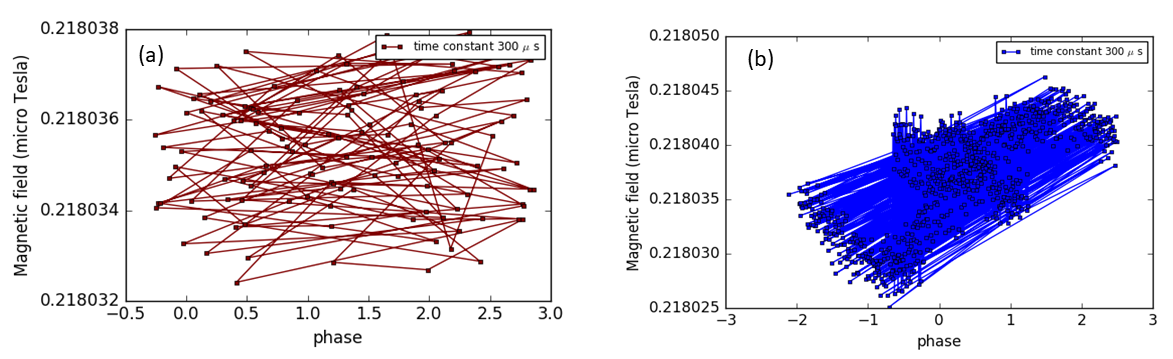
\includegraphics[width=0.8\linewidth]{figures/phase}
\caption{Measured magnetic field as a function of phase for different lock-in reference frequency. The red curve represents measured magnetic field when reference frequency was set to 2015 Hz and the blue data points indicates field for lock-in reference frequency 1943.9 Hz.}
\end{figure} 

 \begin{itemize}
   \item effect of lock-in time constant
   
  A SRS-830 lock-in amplifier is used to grab FID NMOR signal which was connected to the output of balanced photodiode. Table \ref{tab:FID_setting} represents all settings for FID NMOR. In this study the systematic effect of changing locking amplifier time constant on magnetic field measurement has been discussed.
   \begin{figure}
    \centering
    \begin{subfigure}[b]{0.45\textwidth}
        \centering
        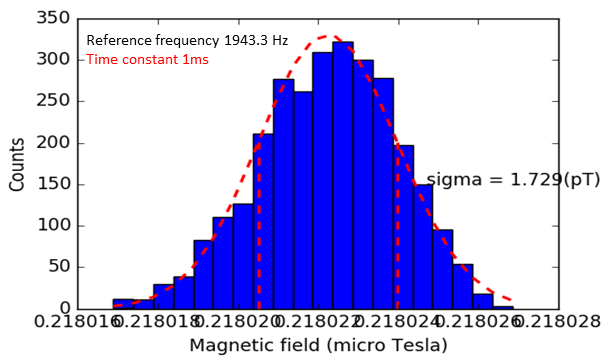
\includegraphics[width=\textwidth]{figures/time_constant}
        \caption{}
        \label{fig:time constant long}
    \end{subfigure}
    \hfill
    \begin{subfigure}[b]{0.45\textwidth}
        \centering
        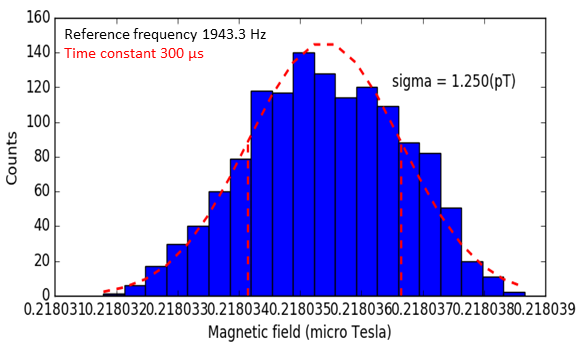
\includegraphics[width=\textwidth]{figures/time_constant_300micro_sec}
        \caption{}
        \label{fig:time constant short}
    \end{subfigure}
    \caption{Histogram of measured magnetic field for different time constant of lock-in amplifier. (a) lock-in time constant was set to 1 ms (b) for lock-in time constant 300 $\mu$s. \label{fig:different time constant} }
\end{figure}
  
  Fig \ref{fig:different time constant}  shows the histogram of measured magnetic field for two different time constant of lock-in amplifier while all other settings is same. In the case of Fig \ref{fig:time constant long} the lock-in time constant is 1 ms and Fig \ref{fig:time constant short} shows the histogram of magnetic field for time constant 300 $\mu$s. Here sigma is representing the precession width of field. It can be seen from the figure that the calculated sigma is larger for time constant 1 ms compared to 300 $\mu$s.  This measurements was conducted at 0.2 $\mu$T field. The resonance frequency and lock-in reference frequency are 2035 Hz and 1943 Hz respectively. The same study has also been done for higher lock-in reference frequency while resonance frequency was unchanged (2035 Hz). Fig: \ref{fig:diff time constant_high_frequency} display the histogram of the recorded magnetic field for different settings of time constant.
  
    \item timing drift in Tektronix oscilloscope clock
   \end{itemize}
   \begin{figure}
    \centering
    \begin{subfigure}[b]{0.45\textwidth}
        \centering
        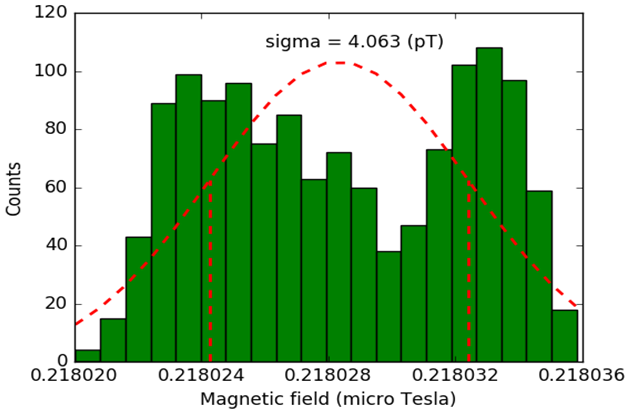
\includegraphics[width=\textwidth]{figures/2015_1ms.png}
        \caption{}
        \label{fig:time constant 1ms}
    \end{subfigure}
    \begin{subfigure}[b]{0.4\textwidth}
        \centering
        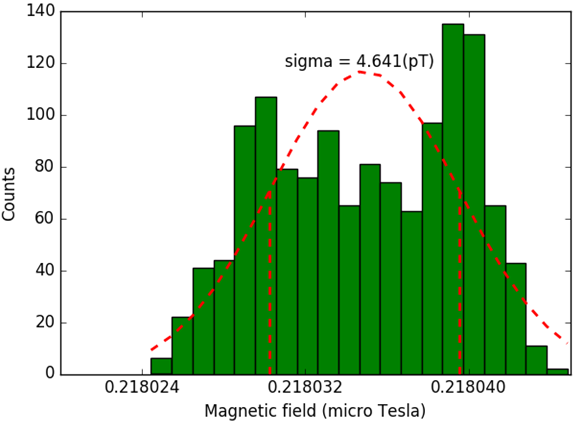
\includegraphics[width=\textwidth]{figures/2015_300micro_sec.png}
        \caption{}
        \label{fig:time constant 300microsec}
    \end{subfigure}
    \caption{Histogram of measured magnetic field for different time constant of lock-in amplifier while lock-in frequency is set to 2015 Hz (20 Hz far from resonance frequency). (a) lock-in time constant was set to 1 ms (b) for lock-in time constant 300 $\mu$s. \label{fig:diff time constant_high_frequency} }
\end{figure}


%The magnetometric method based on FID NMOR is a very sensitive
%technique of magnetic field measurements. Those measurements are
%scalar, i.e., the position of a given resonance depends only on the
%magnitude not the direction of the magnetic field. However, the
%relative magnitudes of the FID NMOR resonances could have some
%dependency on the magnetic field direction. Thus there is a
%possibility to get some information about the direction of the
%magnetic field by doing a detailed analysis of the FID NMOR signal.
%For this reason, the dependency of the FID NMOR signal on the
%magnetic field direction has studied here.
\section{Study magnetometer performance with tilted field} 
\label{sec:tilted-results}
 \begin{figure}
    \centering
    \begin{subfigure}[b]{0.45\textwidth}
        \centering
        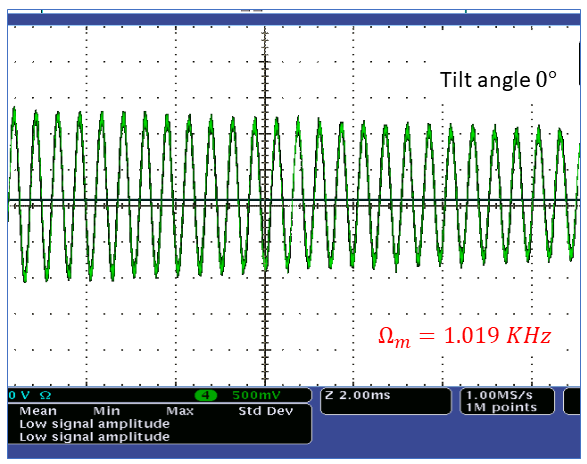
\includegraphics[width=\textwidth,trim={0cm 0.5cm 0cm 0cm},clip]{figures/tilt1.png}
        \caption{}
        \label{fig:tilt_0_degree}
    \end{subfigure}
    \hfill
    \begin{subfigure}[b]{0.45\textwidth}
        \centering
        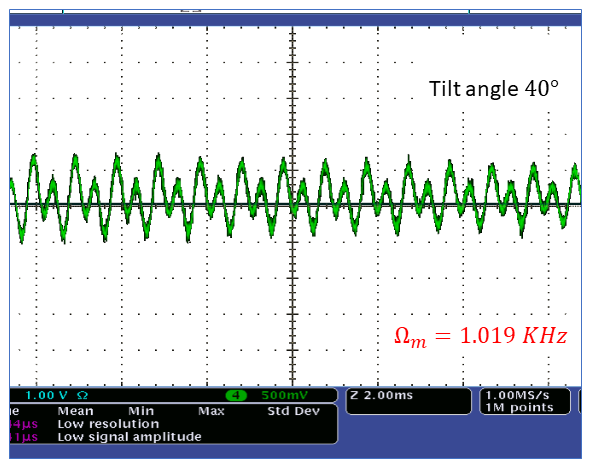
\includegraphics[width=\textwidth,trim={0.7cm 0.5cm 0cm 0cm},clip]{figures/tilt2.png}
        \caption{}
        \label{fig:tilt_40_degree}
    \end{subfigure}
    \begin{subfigure}[b]{0.45\textwidth}
        \centering
        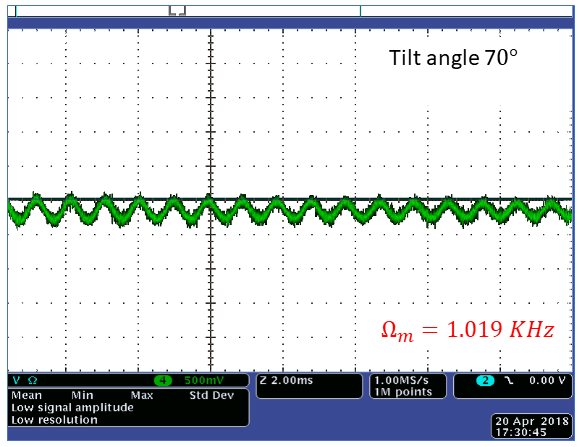
\includegraphics[width=\textwidth,trim={0cm 0.5cm 3.2cm 0cm},clip]{figures/tilt3.png}
        \caption{}
        \label{fig:tilt_70_degree}
    \end{subfigure}
     \hfill
    \begin{subfigure}[b]{0.45\textwidth}
        \centering
        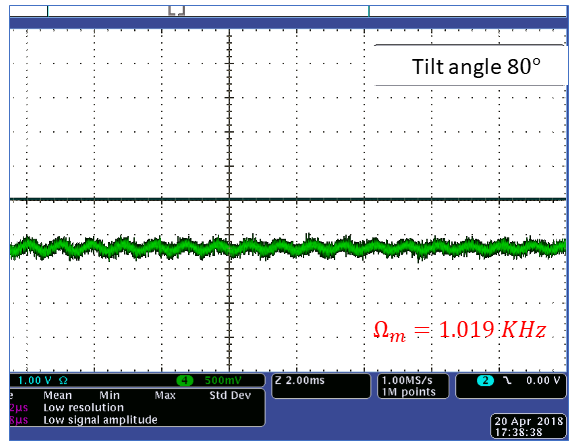
\includegraphics[width=\textwidth,trim={0.5cm 0.5cm 2.9cm 0cm},clip]{figures/tilt4.png}
        \caption{}
        \label{fig:tilt_80_degree}
    \end{subfigure}
    \caption{Optical rotation as a function of time at $\Omega_L$ in the yz plane for different tilt angle.\label{fig:optical-rotation-different-angle}}
\end{figure}
\begin{figure}
  \centering
%trim={<left> <lower> <right> <upper>}
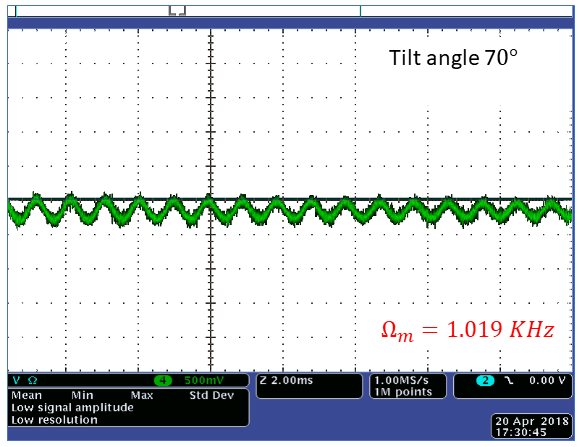
\includegraphics[width=\textwidth,trim={0cm 5.7cm 4.1cm 4.3cm},clip]{figures/tilt3}
 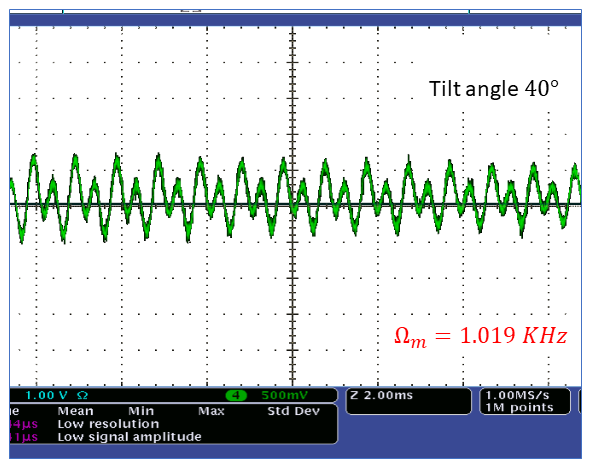
\includegraphics[width=\textwidth,trim={0cm 5cm 0cm 3.5cm},clip]{figures/tilt2}
  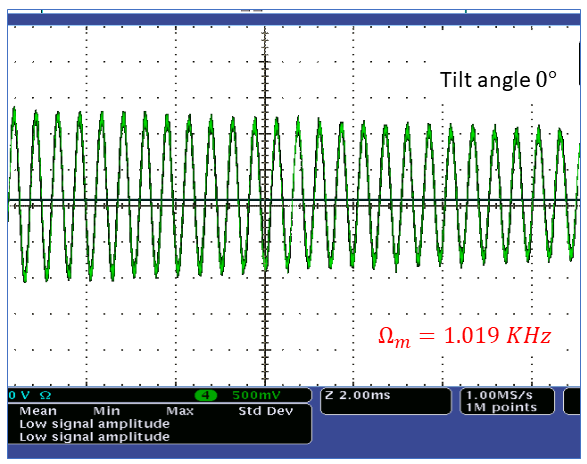
\includegraphics[width=\textwidth,trim={0.4cm 4.5cm 1.7cm 3cm},clip]{figures/tilt1}
  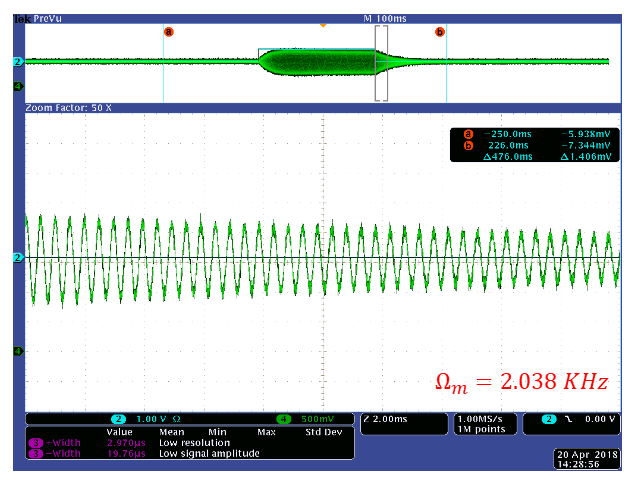
\includegraphics[width=\textwidth,trim={0.4cm 0cm 0.5cm 10.9cm},clip]{figures/transversefield}
  
  \caption{(a) Optical rotation as a function of time at $\Omega_L$ in
    the yz plane at tilt angle $15\degree$ with light propagation
    direction. (b) Optical rotation as a function of time at
    $2\Omega_L$ for same tilt angle.}
    \label{fig:tilted}
\end{figure}
In this Rb NMOR magnetometry setup the rubidium atoms interacted with a $z$-directed laser light beam which is linearly polarized
along the y axis. In the FID NMOR technique, the magnetic field is generally directed along the light propagation direction and the resonance occurs at $2\Omega_L$.  This effect can be explained by considering that the polarization returns to its original state after a $180\degree$ rotation because of the two-fold symmetry of the optically pumped state. As a result, the optical rotation induced by the rotating linear dichroism is periodic at twice the Larmor frequency.

We have observed that Resonances in nonlinear magneto-optical rotation with amplitude modulated light by tilting the magnetic field at angles away from the direction of light propagation while operating the Rb magnetometer in FID mode. When the field is tilted in the plane perpendicular to the light polarization direction an resonance appears at $2\Omega_L$. In this case no additional resonance appears for modulation frequency $\Omega_L$. The amplitude of the FID NMOR signal decreases with increasing tilt angle. 

However, We also observed that by tilting the field direction toward the light polarization direction a new resonance occurs at $\Omega_L$ along with the main resonance at $2\Omega_L$. The resonance signal recorded at $\Omega_L$ contains two frequency components.
\begin{figure}[h]
\centering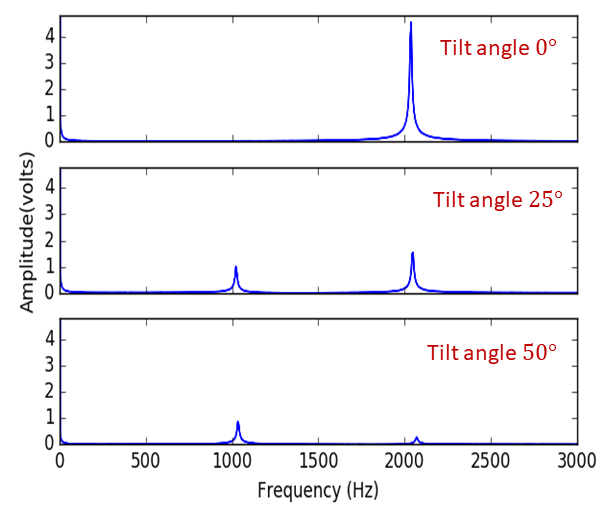
\includegraphics[width=0.7\linewidth]{figures/fft_amp.png}
\caption{FFT of FID  signal in the presence of transverse field at modulation frequency $\Omega_L$ while tilted the magnetic field direction toward light polarization direction  .\label{fig:fft-amplitude}}
\end{figure}


When direction of the magnetic is tilted toward the light polarization axis  the FID signal contain two frequency component at modulation frequency $\Omega_L$. Fig: \ref{fig:optical-rotation-different-angle} shows the FID signal for different tilt angle when pump beam is modulated at $\Omega_L$. In order to extract frequency components we have used two methods. One of them is the FFT of FID signal and the other one is the fit FID signal using equation \ref{eq:two_sinewave}.

\begin{equation}
     X = A_1 e^{-t /\tau_1} \sin(\omega_1 t + \phi_1) + A_2 e^{-t /\tau_2}  \sin (\omega_2 t + \phi_2) + C  
     \label{eq:two_sinewave}
\end{equation}

Where $A_1$ and $A_2$ are amplitude for two decaying sin wave, $\omega_1$ and $\omega_2$ represents oscillation frequency, $\phi_1$ and $\phi_2$ indicate phase and $\tau_1$ and $\tau_2$ represents coherence time. A 10th order Infinite Impulse Response( IIR) Butterworth filter is also used to reduce background noise from the signal.
Fig: \ref{fig:fft-amplitude} display the FFT of resonance signal for three different  tilt angle $0\degree$, $25\degree$ and $50\degree$. It can be seen from the plot that at $0\degree$ tilt angle there is only one frequency component while for $25\degree$ tilt angle two peak corresponds to two frequency components.

Fig.~\ref{fig:tilted-wrong} shows the amplitude of the FID signal for the magnetic field tilted in the $xz$ plane at various angles to the light propagation direction at modulation frequency $2\Omega_L$ and $\Omega_L$. It can be seen from the figure that the amplitude of the FID signal decreases with increasing tilt angle for both modulation frequency. 

\begin{figure}
    \centering
   \begin{subfigure}[b]{0.45\textwidth}
        \centering
        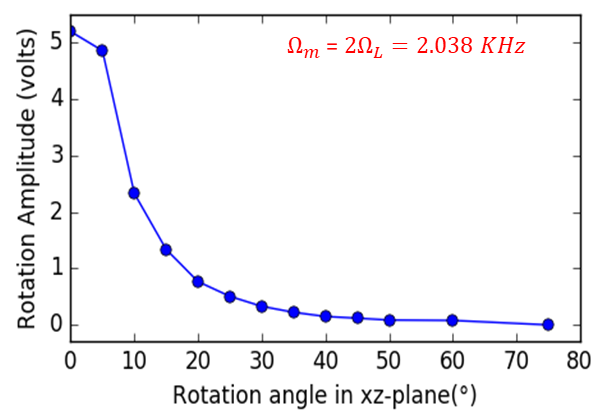
\includegraphics[width=\textwidth]{figures/tilt_x_larmor.png}
        \caption{}
        \label{fig:y equals x}
    \end{subfigure}
    \hfill
     \begin{subfigure}[b]{0.45\textwidth}
        \centering
        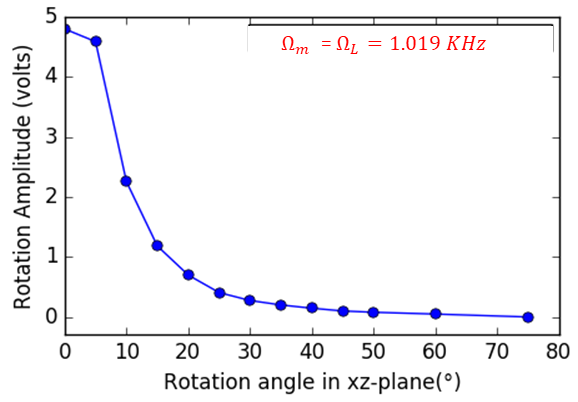
\includegraphics[width=\textwidth]{figures/tilt_x_2larmor.png}
        \caption{}
        \label{fig:three sin x}
    \end{subfigure}
    \caption{ The amplitude of the FID NMOR signals as a function
      of tilt angle recorded at $\Omega_L$ and $2\Omega_L$ vs. the
      tilt angle of the magnetic field in the plane defined by the
      light-polarization and light propagation vectors(xz-plane). \label{fig:tilted-wrong}}
\end{figure}

\begin{figure}
    \centering
   \begin{subfigure}[b]{0.45\textwidth}
        \centering
        \includegraphics[width=\textwidth]{figures/tilt_y_larmor.png}
        \caption{}
        \label{fig:tilt_y}
    \end{subfigure}
    \hfill
     \begin{subfigure}[b]{0.45\textwidth}
        \centering
        \includegraphics[width=\textwidth]{figures/tilt_y_2larmor.png}
        \caption{}
        \label{fig:tilt_x}
    \end{subfigure}
    \caption{(a) The amplitude of the FID NMOR signals as a function
      of tilt angle recorded at $\Omega_L$ and $2\Omega_L$ vs. the
      tilt angle of the magnetic field in the plane defined by the
      light-polarization and light propagation vectors(yz-plane). \label{fig:something-tilted}}
\end{figure}

Fig.~\ref{fig:something-tilted}(a) indicates the signal amplitude vs. different tilt angle at $\Omega_m=2\Omega_L$ . The amplitude of resonance signal at $2\Omega_L$  decreases as the angle between magnetic field $B$ and the light propagation direction increases while the amplitude of new resonance  increases with increasing tilt angle at $\Omega_L$.
      
Fig.~\ref{fig:something-tilted}(b) shows the resonance amplitude at $\Omega_m=2\Omega_L$ keep decreases with increasing tilt angle in $yz$ plane while  the resonance amplitude measured at $\Omega_m=\Omega_L$ keep increase till $30\degree$ and after that amplitude start to decrease and reaches zero when the magnetic field is directed along the y axis. Consider a two-level system $F=1\rightarrow F=0$ and the quantization vector is directed along the magnetic field. When the magnetic field is tilted in the yz plane, the light-polarization axis is perpendicular to the magnetic field. In this case the linearly polarized light containing two circularly polarized components can only create the coherence state between magnetic sublevels $m_F=\pm 1$ . Since the transition frequency between these two consecutive Zeeman energy sublevels is $2\Omega_L$  the resonance appears only at this frequency. However, when the magnetic field is tilted  in the xy plane, the light is a linear superposition of polarizations parallel and perpendicular to the magnetic field. In this case, the light can create coherences between sublevels with $m_F=1$ and $m_F=2$, so resonances are observed at both $\Omega_L $ and $2\Omega_L$. 
 \begin{figure}[h]
\centering\includegraphics[width=0.9\linewidth]{figures/filtered_data.png}
\caption{Raw and filtered FID signal.}
\end{figure}
 

